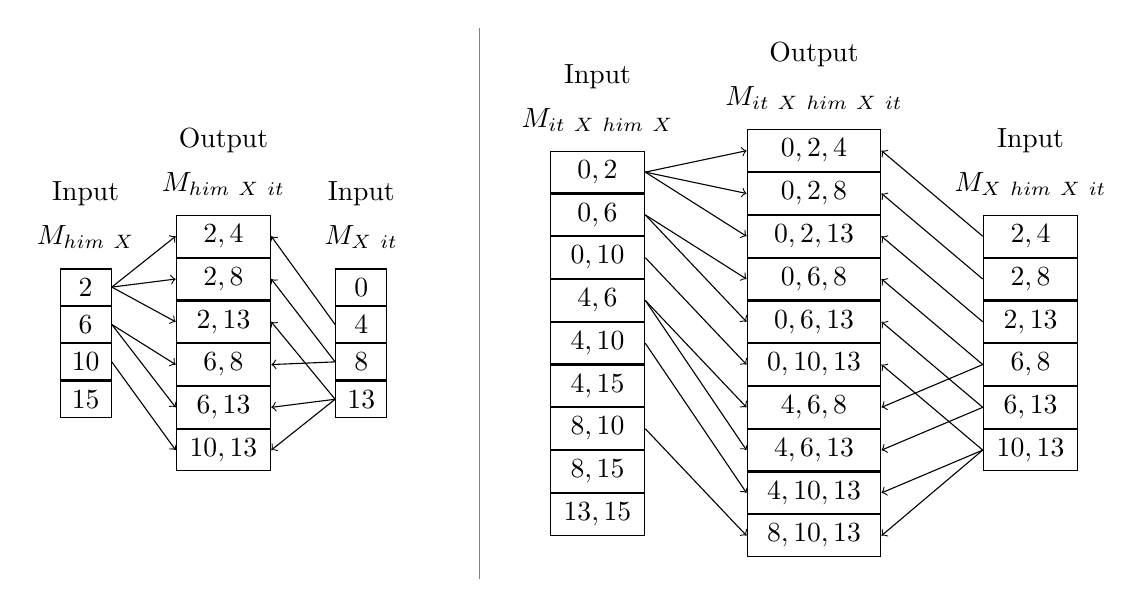
\begin{tikzpicture}[node distance=2.25cm]
	\matrix (him locations) [nodes={rectangle,draw,minimum width=6.5mm}]{
		\node (index 2)  {2}; \\
		\node (index 6)  {6}; \\
		\node (index 10) {10}; \\
		\node (index 15) {15}; \\
	};


	\matrix (him X it locations) [nodes={rectangle,draw,minimum width=12mm},right of=him locations,node distance=1.75cm]{
		\node (index 2 4)   {$2, 4$}; \\
		\node (index 2 8)   {$2, 8$}; \\
		\node (index 2 13)  {$2, 13$}; \\
		\node (index 6 8)   {$6, 8$}; \\
		\node (index 6 13)  {$6, 13$}; \\
		\node (index 10 13) {$10, 13$}; \\
	};


	\matrix (it locations) [nodes={rectangle,draw,minimum width=6.5mm},right of=him X it locations,node distance=1.75cm]{
		\node (index 0)  {0}; \\
		\node (index 4)  {4}; \\
		\node (index 8)  {8}; \\
		\node (index 13) {13}; \\
	};
	
	\node (him label) [anchor=south] at (him locations.north) {$M_{him~X}$};
	\node (pair label) [anchor=south] at (him X it locations.north) {$M_{him~X~it}$};
	\node (it label) [anchor=south] at (it locations.north) {$M_{X~it}$};
	\node [anchor=south] at (him label.north) {Input};
	\node [anchor=south] at (pair label.north) {Output};
	\node [anchor=south] at  (it label.north) {Input};

	\draw[->] (index 2.east) -- (index 2 4.west);
	\draw[->] (index 2.east) -- (index 2 8.west);
	\draw[->] (index 2.east) -- (index 2 13.west);
	\draw[->] (index 6.east) -- (index 6 8.west);
	\draw[->] (index 6.east) -- (index 6 13.west);
	\draw[->] (index 10.east) -- (index 10 13.west);

	\draw[->] (index 4.west) -- (index 2 4.east);
	\draw[->] (index 8.west) -- (index 2 8.east);
	\draw[->] (index 8.west) -- (index 6 8.east);
	\draw[->] (index 13.west) -- (index 2 13.east);
	\draw[->] (index 13.west) -- (index 6 13.east);
	\draw[->] (index 13.west) -- (index 10 13.east);

	\node (between)[right of=it locations,node distance=1.5cm] {};
	\draw[gray,thin] (between.center) -- +(0cm, 4cm);
	\draw[gray,thin] (between.center) -- +(0cm,-3cm);

	\matrix (it X him locations) [nodes={rectangle,draw,minimum width=12mm},right of=it locations,node distance=3cm]{
		\node (index 0 2)   {$0,2$}; \\
		\node (index 0 6)   {$0,6$}; \\
		\node (index 0 10)   {$0,10$}; \\
		\node (index 4 6)   {$4,6$}; \\
		\node (index 4 10)   {$4,10$}; \\
		\node (index 4 15)   {$4,15$}; \\
		\node (index 8 10)   {$8,10$}; \\
		\node (index 8 15)   {$8,15$}; \\
		\node (index 13 15)  {$13,15$}; \\
	};

	\matrix (it X him X it locations) [nodes={rectangle,draw,minimum width=17mm},right of=it X him locations,node distance=2.75cm]{
		\node (index 0 2 4)  {$0,2,4$}; \\
		\node (index 0 2 8)  {$0,2,8$}; \\
		\node (index 0 2 13)  {$0,2,13$}; \\
		\node (index 0 6 8)  {$0,6,8$}; \\
		\node (index 0 6 13)  {$0,6,13$}; \\
		\node (index 0 10 13)  {$0,10,13$}; \\
		\node (index 4 6 8)  {$4,6,8$}; \\
		\node (index 4 6 13)  {$4,6,13$}; \\
		\node (index 4 10 13)  {$4,10,13$}; \\
		\node (index 8 10 13)  {$8,10,13$}; \\
	};


	\matrix (him X it locations) [nodes={rectangle,draw,minimum width=12mm},right of=it X him X it locations,node distance=2.75cm]{
		\node (index 2 4)   {$2, 4$}; \\
		\node (index 2 8)   {$2, 8$}; \\
		\node (index 2 13)  {$2, 13$}; \\
		\node (index 6 8)   {$6, 8$}; \\
		\node (index 6 13)  {$6, 13$}; \\
		\node (index 10 13) {$10, 13$}; \\
	};

	\node (him label) [anchor=south] at (him X it locations.north) {$M_{X~him~X~it}$};
	\node (pair label) [anchor=south] at (it X him X it locations.north) {$M_{it~X~him~X~it}$};
	\node (it label) [anchor=south] at (it X him locations.north) {$M_{it~X~him~X}$};
	\node [anchor=south] at (him label.north) {Input};
	\node [anchor=south] at (pair label.north) {Output};
	\node [anchor=south] at  (it label.north) {Input};

	\draw[->] (index 0 2.east) -- (index 0 2 4.west);
	\draw[->] (index 0 2.east) -- (index 0 2 8.west);
	\draw[->] (index 0 2.east) -- (index 0 2 13.west);
	\draw[->] (index 0 6.east) -- (index 0 6 8.west);
	\draw[->] (index 0 6.east) -- (index 0 6 13.west);
	\draw[->] (index 0 10.east) -- (index 0 10 13.west);
	\draw[->] (index 4 6.east) --  (index 4 6 8.west);
	\draw[->] (index 4 6.east) --  (index 4 6 13.west);
	\draw[->] (index 4 10.east) -- (index 4 10 13.west);
	\draw[->] (index 8 10.east) -- (index 8 10 13.west);

	\draw[->] (index 2 4.west) -- (index 0 2 4.east);
	\draw[->] (index 2 8.west) -- (index 0 2 8.east);
	\draw[->] (index 2 13.west) -- (index 0 2 13.east);
	\draw[->] (index 6 8.west) --  (index 0 6 8.east);
	\draw[->] (index 6 13.west) -- (index 0 6 13.east);
	\draw[->] (index 6 8.west) --  (index 4 6 8.east);
	\draw[->] (index 6 13.west) -- (index 4 6 13.east);
	\draw[->] (index 10 13.west) -- (index 0 10 13.east);
	\draw[->] (index 10 13.west) -- (index 4 10 13.east);
	\draw[->] (index 10 13.west) -- (index 8 10 13.east);

\end{tikzpicture}





